\documentclass[%
	paper=A4,	% stellt auf A4-Papier
	pagesize,	% gibt Papiergröße weiter
	DIV=calc,	% errechnet Satzspiegel
	smallheadings,	% kleinere Überschriften
	ngerman		% neue Rechtschreibung
]{scrartcl}
\usepackage{BenMathTemplate}
\usepackage{BenTextTemplate}

\title{{\bf Wissenschaftliches Rechnen III / CP III}\\Übungsblatt 4}
\author{Tizia Kaplan (545978)\\Benjamin Dummer (532716)}
\date{25.05.2016}

\begin{document}
\maketitle
Online-Version: \href{https://www.github.com/BeDummer/CP3_UE4}{\url{https://www.github.com/BeDummer/CP3_UE4}}

\section*{Aufgabe 4.1}

\begin{figure}
  \centering
  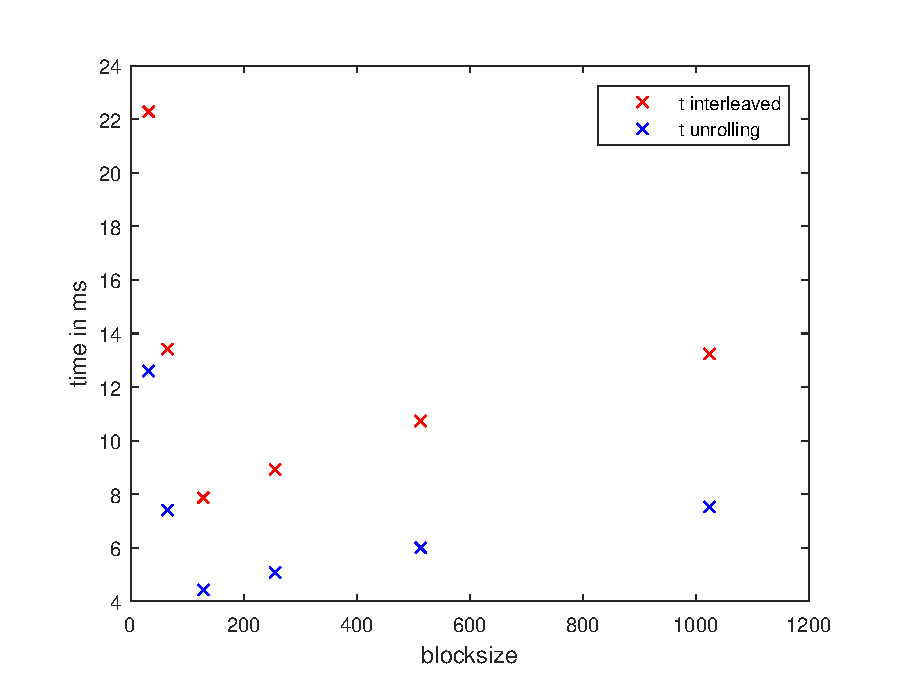
\includegraphics[width=.8\textwidth]{blocksize_vs_time_interl_unroll.eps}
  \caption{Blocksize vs. Simulationszeit f"ur die unterschiedlichen Realisierungen der parallelen Reduktion (interleaved \& unroll)}
\end{figure}

\begin{figure}
  \centering
  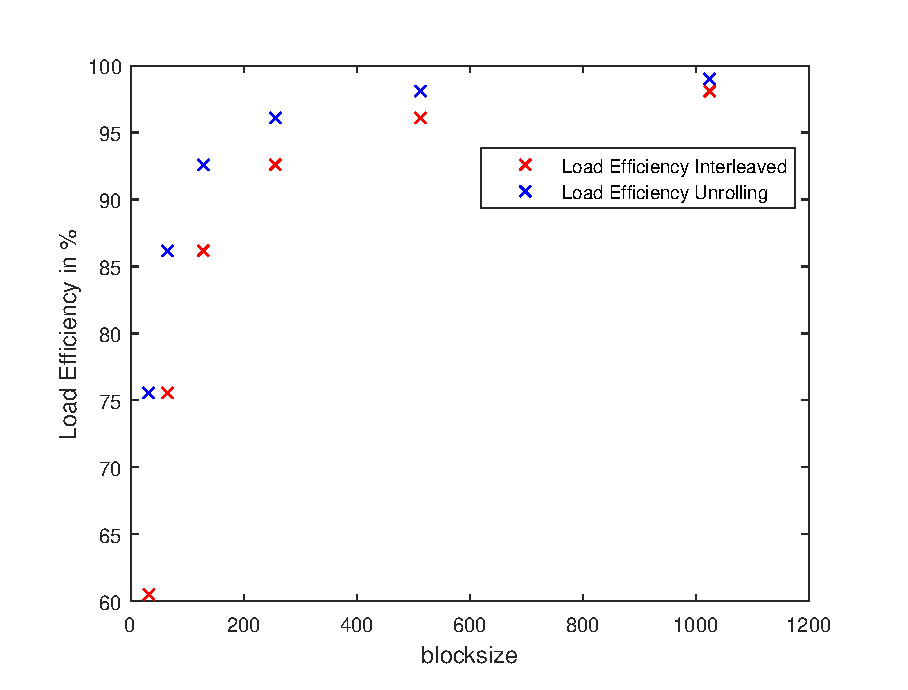
\includegraphics[width=.8\textwidth]{blocksize_vs_load_efficiency.eps}
  \caption{Blocksize vs. Global Load Efficiency f"ur die unterschiedlichen Realisierungen der parallelen Reduktion (interleaved \& unroll)}
\end{figure}

\begin{figure}
  \centering
  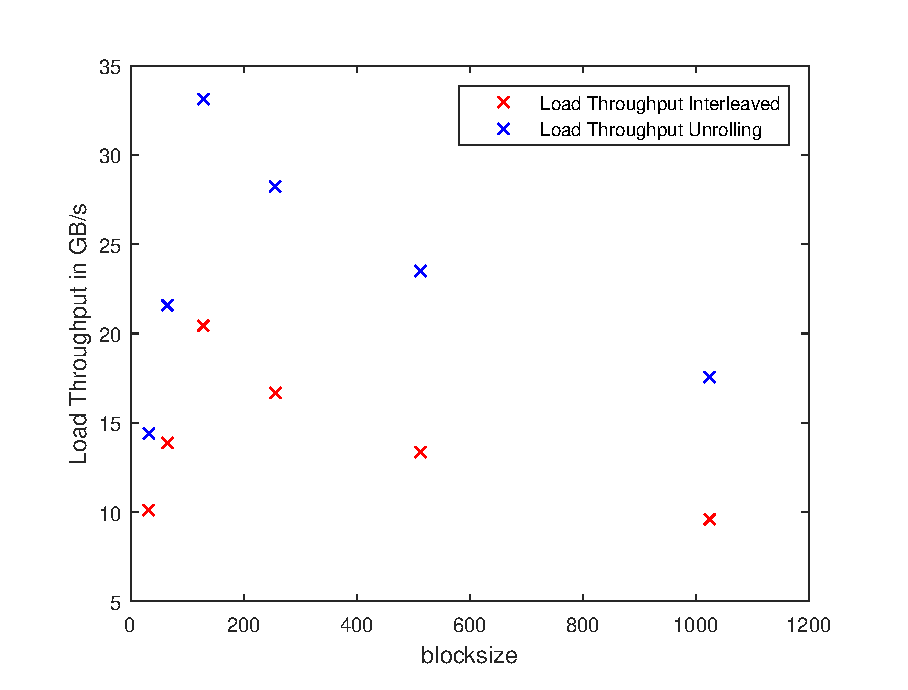
\includegraphics[width=.8\textwidth]{blocksize_vs_load_throughput.eps}
  \caption{Blocksize vs. Global Load Throughput (Bandbreite) f"ur die unterschiedlichen Realisierungen der parallelen Reduktion (interleaved \& unroll)}
\end{figure}

\begin{figure}
  \centering
  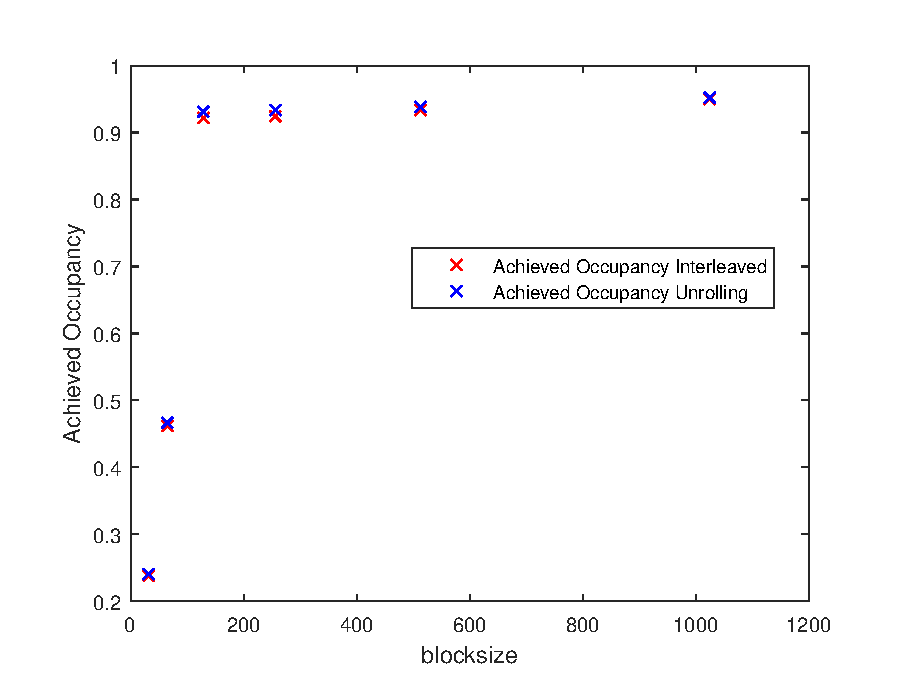
\includegraphics[width=.8\textwidth]{blocksize_vs_achieved_occ.eps}
  \caption{Blocksize vs. Achieved Occupancy f"ur die unterschiedlichen Realisierungen der parallelen Reduktion (interleaved \& unroll)}
\end{figure}

\section*{Anhänge}
\begin{itemize}
	\item Datei: \url{reduction_w_q.cu} (Hauptprogramm)
\end{itemize}
\end{document}
